\chapter{Another chapter}\label{ch:results}

\section{Ground State Degeneracy}
In this chapter results of simulations on the dipolar kagome lattice are presented. EFM simulations reveal a many-fold degenerate ground state allowing zero-temperature states that consist of six unique spins. Ground states obtained through the EFM simulation exhibit a six-sublattice structure; three of the sublattices contain spins that are the negatives of the spins on the remaining three sublattices. The spins alternate in direction along the [1,1,1] direction.

\begin{figure}
	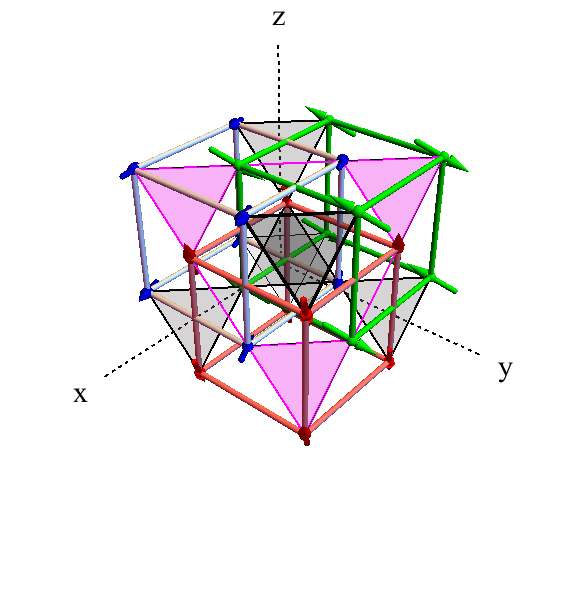
\includegraphics[width=\linewidth]{img/3dfcc.png}
	\caption{A view down the <1,1,1> axis of a 3D FCC lattice with six sub-lattice spin vectors.}
	\label{fig:3dfcc}
\end{figure}

\clearpage
Every ground state configuration obtained through the EFM simulation is characterized by the following set of equations:
\begin{equation}
\label{eqn:rel_a}
\alpha = \sin{\theta} \cos{\phi}
\end{equation}
\begin{equation}
\label{eqn:rel_b}
\beta = \sin{\theta} \sin{\phi}
\end{equation}
\begin{equation}
\label{eqn:rel_c}
\chi = \cos{\theta}
\end{equation}
\begin{equation}
\label{eqn:rel_d}
\delta = (2a^2-1)/2c
\end{equation}
\begin{equation}
\label{eqn:rel_e}
\epsilon = \sqrt(1-a^2-d^2)
\end{equation}

This set of equations acts as elementary building blocks for the components of the spin vectors that exist in the dipolar kagome ground state. There are two parameters that dictate the resulting ground state: $\theta$ and $\phi$, which are polar angles of the spin "A". Spin A is arbitrarily chosen. The spin vectors themselves may be constructed as follows:

$$\overrightarrow{a} = (\alpha, \beta, \chi)$$
$$\overrightarrow{b} = (\delta, \epsilon, -\alpha)$$
$$\overrightarrow{c} = (-\epsilon, -\chi-\delta, \beta)$$
$$\overrightarrow{d} =-\overrightarrow(a)$$
$$\overrightarrow{e} =-\overrightarrow(b)$$
$$\overrightarrow{f} =-\overrightarrow(c)$$

\begin{figure}
	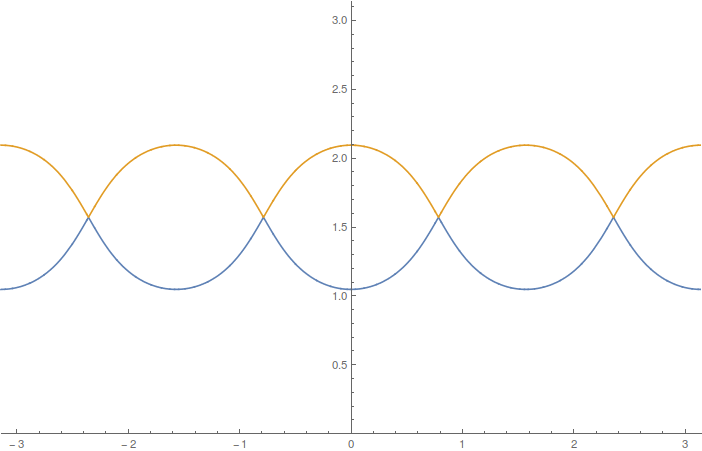
\includegraphics[width=\linewidth]{img/degeneracyplanefull.png}
	\caption{A plane that contains points that allow the construction of valid ground states.}
	\label{fig:degenplanefull}
\end{figure}


Any theta and phi will give rise to a valid ground state of the same energy with the exception of those pairs of theta and phi that lie within the bound region of the graph. Within the bound region of the graph, e = √(1–a²–d²) ∈ ℂ. At each node of each bound area, d = (2a²–1)/2c → ±0/0.

\begin{figure}
	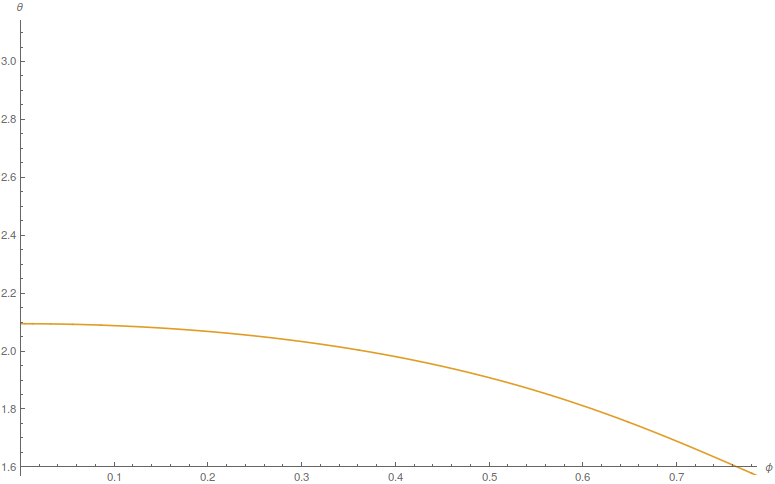
\includegraphics[width=\linewidth]{img/degeneracyplane.png}
	\caption{One section of the original degeneracy plane that is equivalent to all other sections of the plane due to symmetry operations.}
	\label{fig:degenplane}
\end{figure}

It is possible to reduce the size of this graph to 1/16 the size by showing that a state in each portion of the graph is relatable to an analogous state in the other portions of the graph via symmetry operations.
\clearpage

\subsection{Visualization of the Ground State}
\begin{figure}[ht]
	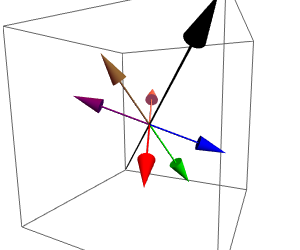
\includegraphics[scale=1.2]{img/samplegs.png}
	\caption{The six sublattice spins conjoined at their ends for clarity and illustration. The vector denoting <1,1,1> axis of symmetry is illustrated in black}
	\label{fig:sampgs}
\end{figure}

By generating the spin vectors described by the !!!equations!!!, spin configurations ranging from planar to non-planar states can be obtained. The following contour plot illustrates the volume of a parallelopiped formed by a spin configuration corresponding to a particular $\theta$ and $\phi$ on the plane of the plot. It is from this illustration that one can obtain an understanding of what choices of $\theta$ and $\phi$ result in planar states or non-planar states.


\begin{figure}[ht]
	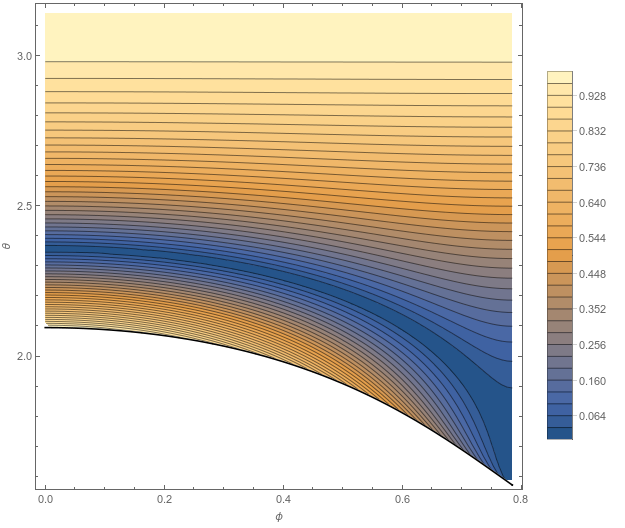
\includegraphics[width=\linewidth]{img/groundstatevol.png}
	\caption{A contour plot of volume of a parallelopiped formed by a spin configuration with respect to $\theta$ and $\phi$ }
	\label{fig:gsvol}
\end{figure}
\clearpage

The following plots illustrate some of the possible spin configurations that result from particular choices of $\theta$ and $\phi$. 

\begin{figure}
	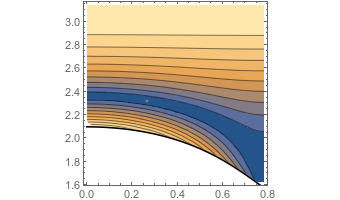
\includegraphics[scale=1]{img/th2-3108_phi0-27_plane.png}
\end{figure}
\begin{figure}
  \begin{minipage}[b]{0.5\linewidth}
    \centering
    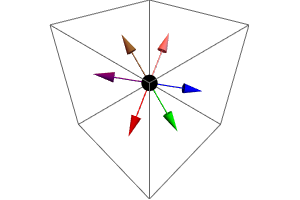
\includegraphics[width=.8\linewidth]{img/th2-3108_phi0-27_view1.png} 
    \caption{View 1} 
    \vspace{4ex}
  \end{minipage}%%
  \begin{minipage}[b]{0.5\linewidth}
    \centering
    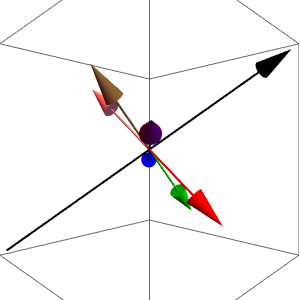
\includegraphics[width=.5\linewidth]{img/th2-3108_phi0-27_view2.png} 
    \caption{View 2} 
    \vspace{4ex}
  \end{minipage} 
  \begin{minipage}[b]{0.5\linewidth}
    \centering
    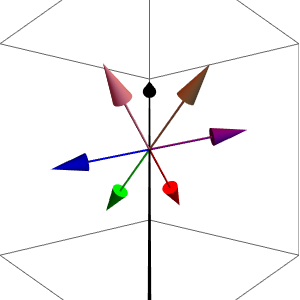
\includegraphics[width=.5\linewidth]{img/th2-3108_phi0-27_view3.png} 
    \caption{View 3} 
    \vspace{4ex}
  \end{minipage}%% 
  \begin{minipage}[b]{0.5\linewidth}
    \centering
    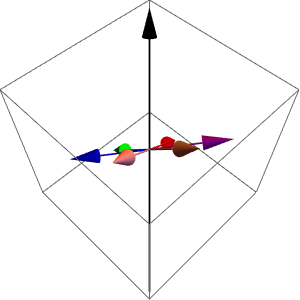
\includegraphics[width=.5\linewidth]{img/th2-3108_phi0-27_view4.png} 
    \caption{View 4} 
    \vspace{4ex}
  \end{minipage} 
\end{figure}

\clearpage
\subsection{Planar Ground States}

The thin strip of blue that cuts into the contour plot just above the complex region consists of the set of points that give rise to parallelopipeds with the smallest volume. This corresponds to spin configurations that are planar. Elsewhere in the plane, the spin configurations are non-planar. The strip of points that give rise to planar states are described by the following polar equations:

\begin{equation}
\phi = \frac{\pi}{4}\cos{\gamma} 
\end{equation}
\begin{equation}
\theta = \frac{\pi}{4}(\sin{\gamma}+2)
\end{equation}

The spin configurations that are planar can therefore be described in terms of one parameter, $\gamma$, the polar equations which determine $\theta$ and $\phi$, and the original set of equations.  

\begin{figure}[h]
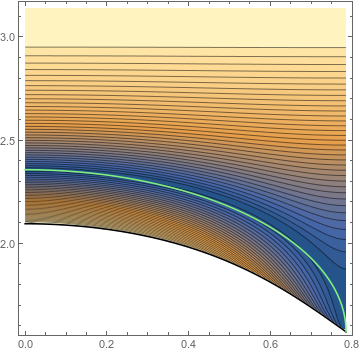
\includegraphics[width=.5\linewidth]{img/groundstatevol_withplanarborder.png} 
    \caption{Contour plot of parallelepiped volume with the perimeter of a circle shown in green.} 
\end{figure}
\clearpage
\section{3D Dipolar Kagome Finite T EFM Results}


\section{3D Dipolar Kagome Magnetic Field EFM Results}

In this section results on application of an external magnetic field on the dipolar kagome lattice are presented. EFM simulations reveal how a sufficiently large external magnetic field causes the spin configuration to transition from a non-planar state to a planar state. Following this transition, the spins undergo a linear change in orientation with respect to magnetic field magnitude by reorienting in the direction of the magnetic field. Following degaussing, the spins will unalign with the magnetic field and form a planar state at zero magnetic field magnitude, regardless of whether the state was initially non-planar. In essence, when degaussing with a sufficiently high peak magnetic field magnitude, any minimum-energy state can be transformed into a planar state. Finally, with sufficiently high magnetic field magnitude, the lattice becomes saturated and the rate at which the spins reorient themselves along the direction of the magnetic field is reduced. 

%Add in:
%Graph of magnetization summarizing the different phases (Get this from your presentation)
%Cube face data for increasing and decreasing magnetic field 
%Cube axis data for increasing and decreasing magnetic field. Get from cumulative june 26/16 latex 
%Saturation stuff, along 111
